\documentclass{article}
\usepackage{tikz}
\usetikzlibrary{shapes.geometric, arrows}

\newcommand{\hash}{\mbox{\tt \#}}
\newcommand{\one}{\mbox{\tt 1}}

\tikzstyle{startstop} = [rectangle, rounded corners, 
minimum width=3cm, 
minimum height=1cm,
text centered, 
draw=black, 
fill=red!30]

\tikzstyle{io} = [trapezium, 
trapezium stretches=true, % A later addition
trapezium left angle=70, 
trapezium right angle=110, 
minimum width=3cm, 
minimum height=1cm, text centered, 
draw=black, fill=blue!30]

\tikzstyle{process} = [rectangle, 
minimum width=3cm, 
minimum height=1cm, 
text centered, 
text width=3cm, 
draw=black, 
fill=orange!30]

\tikzstyle{longprocess} = [rectangle, 
minimum width=4cm, 
minimum height=1cm, 
text centered, 
text width=4cm, 
draw=black, 
fill=orange!30]

\tikzstyle{decision} = [diamond, 
minimum width=3cm, 
minimum height=1cm, 
text centered, 
draw=black, 
fill=green!30]
\tikzstyle{arrow} = [thick,->,>=stealth]
\begin{document}

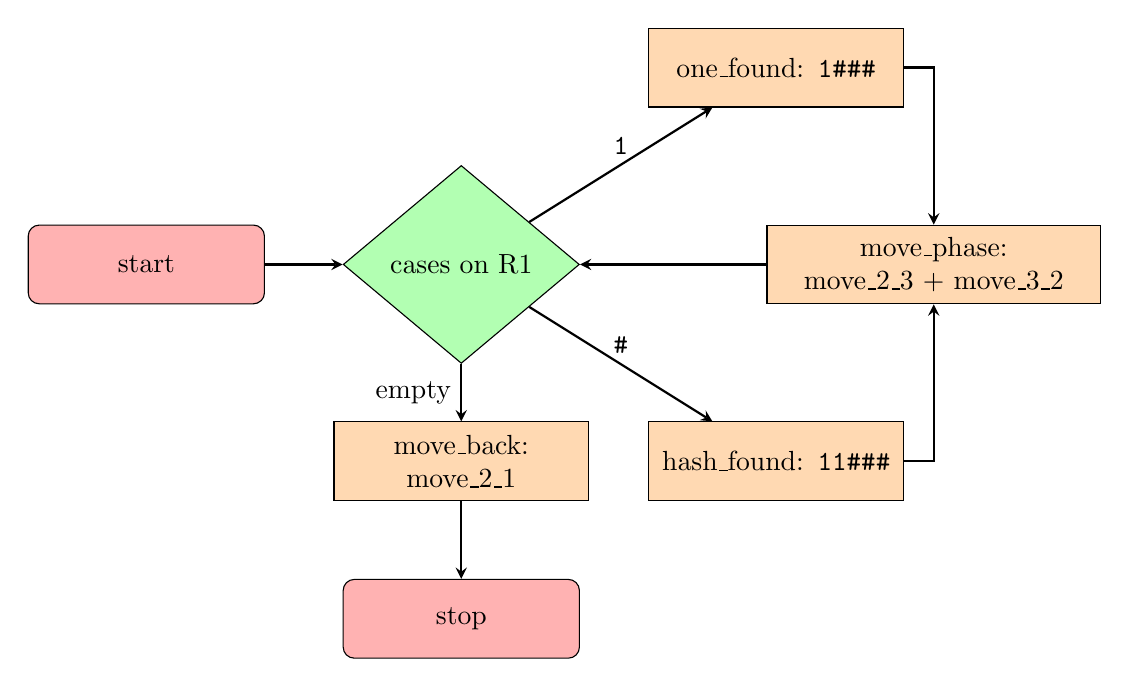
\begin{tikzpicture}[node distance=2cm]


%\node (in1) [io, below of=start] {Input};
%\node (pro1) [process, below of=in1] {move23 + move32};
\node (dec1) [decision, yshift=-0.5cm] {cases on R1};
\node (start) [startstop,left of=dec1, xshift=-2cm] {start};
\node (moveback) [process, below of=dec1, yshift=-0.5cm] {move\_back: \\
move\_2\_1};

\node (onefound) [process, right of=dec1,above of= dec1,xshift=2cm, yshift=.5cm] {one\_found: $\one\hash\hash\hash$};
%\node (out1) [io, below of=pro2a] {Output};
\node (stop) [startstop, below of=moveback] {stop};
\node (hashfound) [process, right of=dec1, below of= dec1,xshift=2cm, yshift=-.5cm] {hash\_found: $\one\one\hash\hash\hash$};
\node (doublemove) [longprocess, right of=dec1, xshift = 4cm] {move\_phase: \\ move\_2\_3 + move\_3\_2};
\draw [arrow] (start) -- (dec1);
%\draw [arrow] (in1) -- (pro1);
%\draw [arrow] (pro1) -- (dec1);
\draw [arrow] (dec1) -- node[anchor=east] {empty} (moveback);
\draw [arrow] (dec1) -- node[anchor=south] {$\mathtt{1}$} (onefound);
\draw [arrow] (dec1) -- node[anchor=south] {{\tt \#}} (hashfound);
%\draw [arrow] (onefound) |- (pro1);
\draw [arrow] (hashfound) -| (doublemove);
\draw [arrow] (onefound) -| (doublemove);
\draw [arrow] (moveback) -- (stop);
\draw [arrow] (doublemove) -- (dec1);
%\draw [arrow] (out1) -- (stop);

\end{tikzpicture}
\end{document}